\documentclass[12pt]{article}

%\usepackage{times} %for Times New Roman, if required
\usepackage[top=1in, bottom=1in, left=1in, right=1in]{geometry} %adjust margins. TODO: hack to fix large top margin
\usepackage{setspace} %allows doublespacing, onehalfspacing, singlespacing
\usepackage{enumitem} %for continuing lists
\usepackage{titling} %for moving the title
\usepackage[normalem]{ulem} %for underlining
\usepackage{graphics}

%redefine section numbering to match Mayron's style
\renewcommand{\thesection}{\arabic{section}} %make sections use numbers
\renewcommand{\thesubsection}{\alph{subsection}} %make subsections use letters
\renewcommand{\thesubsubsection}{\roman{subsubsection}} %subsubsections use romans

\setcounter{tocdepth}{2}

\begin{document}

\begin{spacing}{.4}
\setlength{\droptitle}{-7em}
\title{CSE 485 Semester Report \\  Team 1, Friday 10:30am}
\author{Connor Alfheim \and Ryan Dougherty \and David Ganey \and Dylan Lusi \and Joseph North \and Ben Roos}
\maketitle
\end{spacing}

\begin{spacing}{1.5}
\noindent
Project sponsors: Dr. Judd Bowman and Dr. Danny Jacobs \\
Project description: A virtual observatory for the Murchison Widefield Array radio telescope.
\newpage

\tableofcontents
\newpage

\section{Executive Summary}
The Murchison Widefield Array (MWA) is an enormous radio telescope in Australia used by scientists to monitor hydrogen radiation. This telescope assists scientists interested in learning about the formation of the universe. Erosive, a website which allows scientists to communicate regarding the MWA data, is in need of additional functionality. This project was formed to address the deficits with the current EoRLive website and to allow the scientists to more efficiently engage with their data.

\section{Introduction}
\subsection{Project description}
This semester, we produced a website which functions as a data browser for the MWA telescope's observations. It allows a user to log in with their account and select a date range using selectors at the top of the page and see a list of telescope observations that happened in that range (or scheduled observations that will happen, if the range extends into the future). Specifically, the user can see the observation ID (the unique identifier for the observation in the system), the observation name, and who scheduled the observation. Additionally, the user can see a graph that shows the status of the telescope's data pipeline over that date range. This graph shows the total observation hours scheduled for the telescope versus how many hours have actually been observed, and how many hours' worth of observation data have been transferred from the telescope to databases at MIT.
\subsection{Purpose of project}
The motivation for this project was to make improvements upon the existing site, which lacked some key features the MWA researchers really wanted. They wanted a site that would allow them to monitor the status of the telescope in real time, annotate and share data sets, create discussions about the data through forum-style discussions, and write custom queries that allow them to see the data they want, all on an intuitive Web platform. Ultimately, the goal for this project was to build a more dynamic, collaborative, and customizable site.

\section{Scope}
\subsection{Original Definition}
\subsection{Change of scope and reason for change}

\section{User Overview}
The intended users of this website are astrophysicists involved in research which focuses on monitoring hydrogen radiation throughout the universe. The users are already familiar with the Murchison Widefield Array and the science associated with it. Some of the scientists may be familiar with software development (for example, experience with scripting languages like Python), but it is assumed that none of the users have a deep understanding of software development.

\subsection{Use case diagram}
\subsubsection{Figure 1: User with account}
\begin{center}
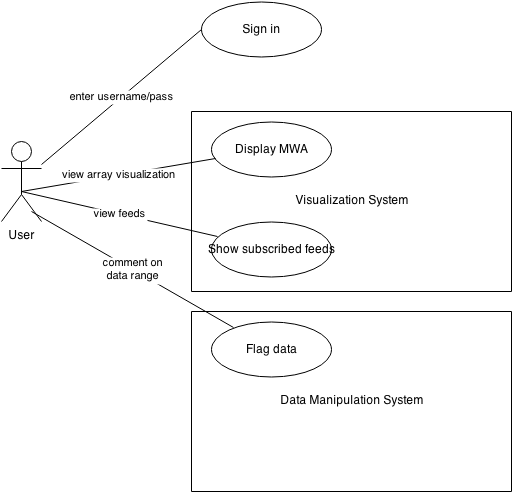
\includegraphics{usecase1} %we can use this to insert .png files in the same directory
\end{center}
\newpage
Users who are not logged in are not permitted to edit the data:
\subsubsection{Figure 2: User without account}
\begin{center}
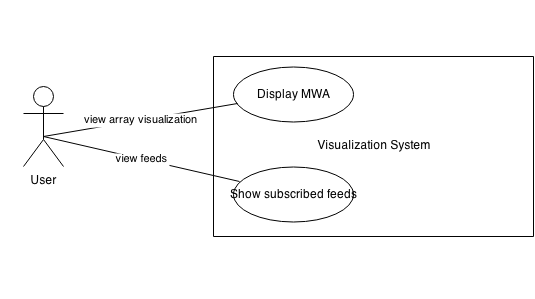
\includegraphics{usecase2}
\end{center}

\subsection{Description of actors}
In the figures above, the actors are viewers of the EoRLive website. The users in Figure 1 are all scientists, and must have been approved by a site admin in order to view the website. The actor in Figure 2 encompasses any user, regardless of affiliation with a specific scientific organization. 

\subsection{User stories}
\begin{enumerate}
\item User views website
	\begin{itemize}
		\item As a user who is not signed in, I want to see a graphical representation of the Murchison Widefield Array so I can tell whether any of the telescope's nodes are malfunctioning.
		\item Given that the data stream is valid, when the user loads the page, the page should show a graphic that shows the state of the array.
	\end{itemize}
\item User signs in
	\begin{itemize}
        		\item As as user with an account, I want to sign in with my account on the site so I can view the site with my custom settings enabled.
        		\item Given that the user's credentials are valid, the website should allow the user to sign in and should load their personal settings before rendering the page.
		\item Given that the user's credentials are invalid, the website should refuse to allow the user to sign in but should still show the status of the array.
	\end{itemize}
\item User modifies settings
	\begin{itemize}
		\item As a signed-in user, I want to modify my subscription settings so I can choose which data streams I will be shown.
		\item Given that the user is signed in, the user should be permitted to modify subscription settings.
		\item Given that the user is not signed in, the user should not be permitted to see or modify subscription settings.
	\end{itemize}
\item User flags data
	\begin{itemize}
		\item As a signed-in user, I want to leave comments on data streams so I can collaborate with other users and generate discussions about the data.
		\item Given that the user is signed in, and that the data stream is valid, the user should be permitted to leave comments on a data stream.
		\item Given that the user is not signed in or that the data stream is not valid, the user should not be permitted to leave comments on that data stream.
	\end{itemize}
\end{enumerate}

\section{Project Plan}

\subsection{First semester}

\subsection{Second Semester}

\section{Development Approach}

\section{Design Overview and Decisions}

\section{Technology and Tools}
\subsection{Programming Languages}
The development for this website uses many of the standard web-development languages. Front-end design is accomplished using HTML and CSS. Some client-side code is run with JavaScript, though this is minimal. The primary server-side language used is Python, in conjunction with a framework called Flask. 

\subsection{Other Tools}
The development environment used by the team is managed by Vagrant. Vagrant is a tool which allows teams to create specific virtual machines, allowing everyone to develop on their own machine but in environments with identical configurations. This allows the team to focus on the code and not on solving issues related to their specific configuration, which can be an issue with web development when users must simulate web servers on their workstations.
\newline \newline
The version control tool chosen to manage our codebase is Git, with GitHub as a host and collaborative tool. Comments and issues on GitHub allow the team to communicate directly on the code. Slack, a team communication tool, was used to keep the development team connected. Standard email communication was used in conjunction with meetings to communicate with the sponsors.

\section{Preliminary results}

\section{Problems and risks}

\section{Summary of Tasks}
\subsection{Connor Alfheim}
\subsubsection{Team Presentation}
\subsubsection{Report}
\subsubsection{Product}
\subsubsection{Initialization Document}
\subsubsection{Team Management}
\subsection{Ryan Dougherty}
\subsubsection{Team Presentation}
\subsubsection{Report}
fdsfsdsdf
\subsubsection{Product}
\subsubsection{Initialization Document}
\subsubsection{Team Management}
\subsection{David Ganey}
\subsubsection{Team Presentation}
\subsubsection{Report}
\subsubsection{Product}
\subsubsection{Initialization Document}
\subsubsection{Team Management}
\subsection{Dylan Lusi}
\subsubsection{Team Presentation}
\subsubsection{Report}
\subsubsection{Product}
\subsubsection{Initialization Document}
\subsubsection{Team Management}
\subsection{Joseph North}
\subsubsection{Team Presentation}
\subsubsection{Report}
\subsubsection{Product}
\subsubsection{Initialization Document}
\subsubsection{Team Management}
\subsection{Ben Roos}
\subsubsection{Team Presentation}
\subsubsection{Report}
fdsfdsa
\subsubsection{Product}
\subsubsection{Initialization Document}
\subsubsection{Team Management}



\section{Conclusions}
\subsection{Success So Far}
\subsection{Lessons Learned}
\subsection{Future Work}


\end{spacing}
\end{document}

